

\section{A note on nuclear physics}

In this thesis we primarily concern ourselves with analysis methods that are agnostic to the physics in the system. One can argue that this is both a strength of the methodology and a weakness. As a consequence the discussion of the physical system will brief. For a more in-depth treatment of the physics  see \cite{Bradt2017}. 

With that in mind we turn to the central pursuits of nuclear physics: understanding the structure of the nucleus. Nuclides are described in terms of the number of protons, $Z$, and neutrons $N$ and their total mass number $A = Z +N$. They are further categorized by equal components; nuclides with an equal number of protons are called \textit{isotopes}, equal number of neutrons \textit{isotones} and with the same  mass \textit{isobars}. The first modern fully-formed theory of nuclear structure, the nuclear shell model, was focused around the observation that certain isotopes and isotones were much more stable than others. As it happened these stable nuclei were regularly spaced around certain numbers of constituent protons and neutrons. These numbers are called magic numbers and describe nuclides that are much more tightly bound than the next number, as a consequence they are very stable and exhibit long half-lives. These magic numbers are: $2 ,\, 8 ,\, 20 ,\, 28 ,\, 50 ,\, 82 ,\, 126$. Some nuclides are even doubly-magic, which is to say both $Z$ and $N$ are magic numbers. One area of active research is around the $N=28$ isotones. Predictions from the nuclear shell model indicates that these isotones should have an approximately spherical structure. This has been disproved experimentally, as deformities appear when removing protons from the spherical nucleus ${}^{48}Ca$. Which brings us to ${}^{46}Ar$ which lies in a region between the spherical ${}^{48}Ca$ and the lighter isotones that are known to be deformed. The location of ${}^{46}Ar$ makes it an object of some academic interest, and served as the commissioning of the AT-TPC at the NSCL. 

% The AT-TPC is a charged particle detector built at the NSCL designed to capture events in the energy range $0.3\mega \eV \per u$ to  $6\mega \eV \per u$

\begin{figure}
\centering
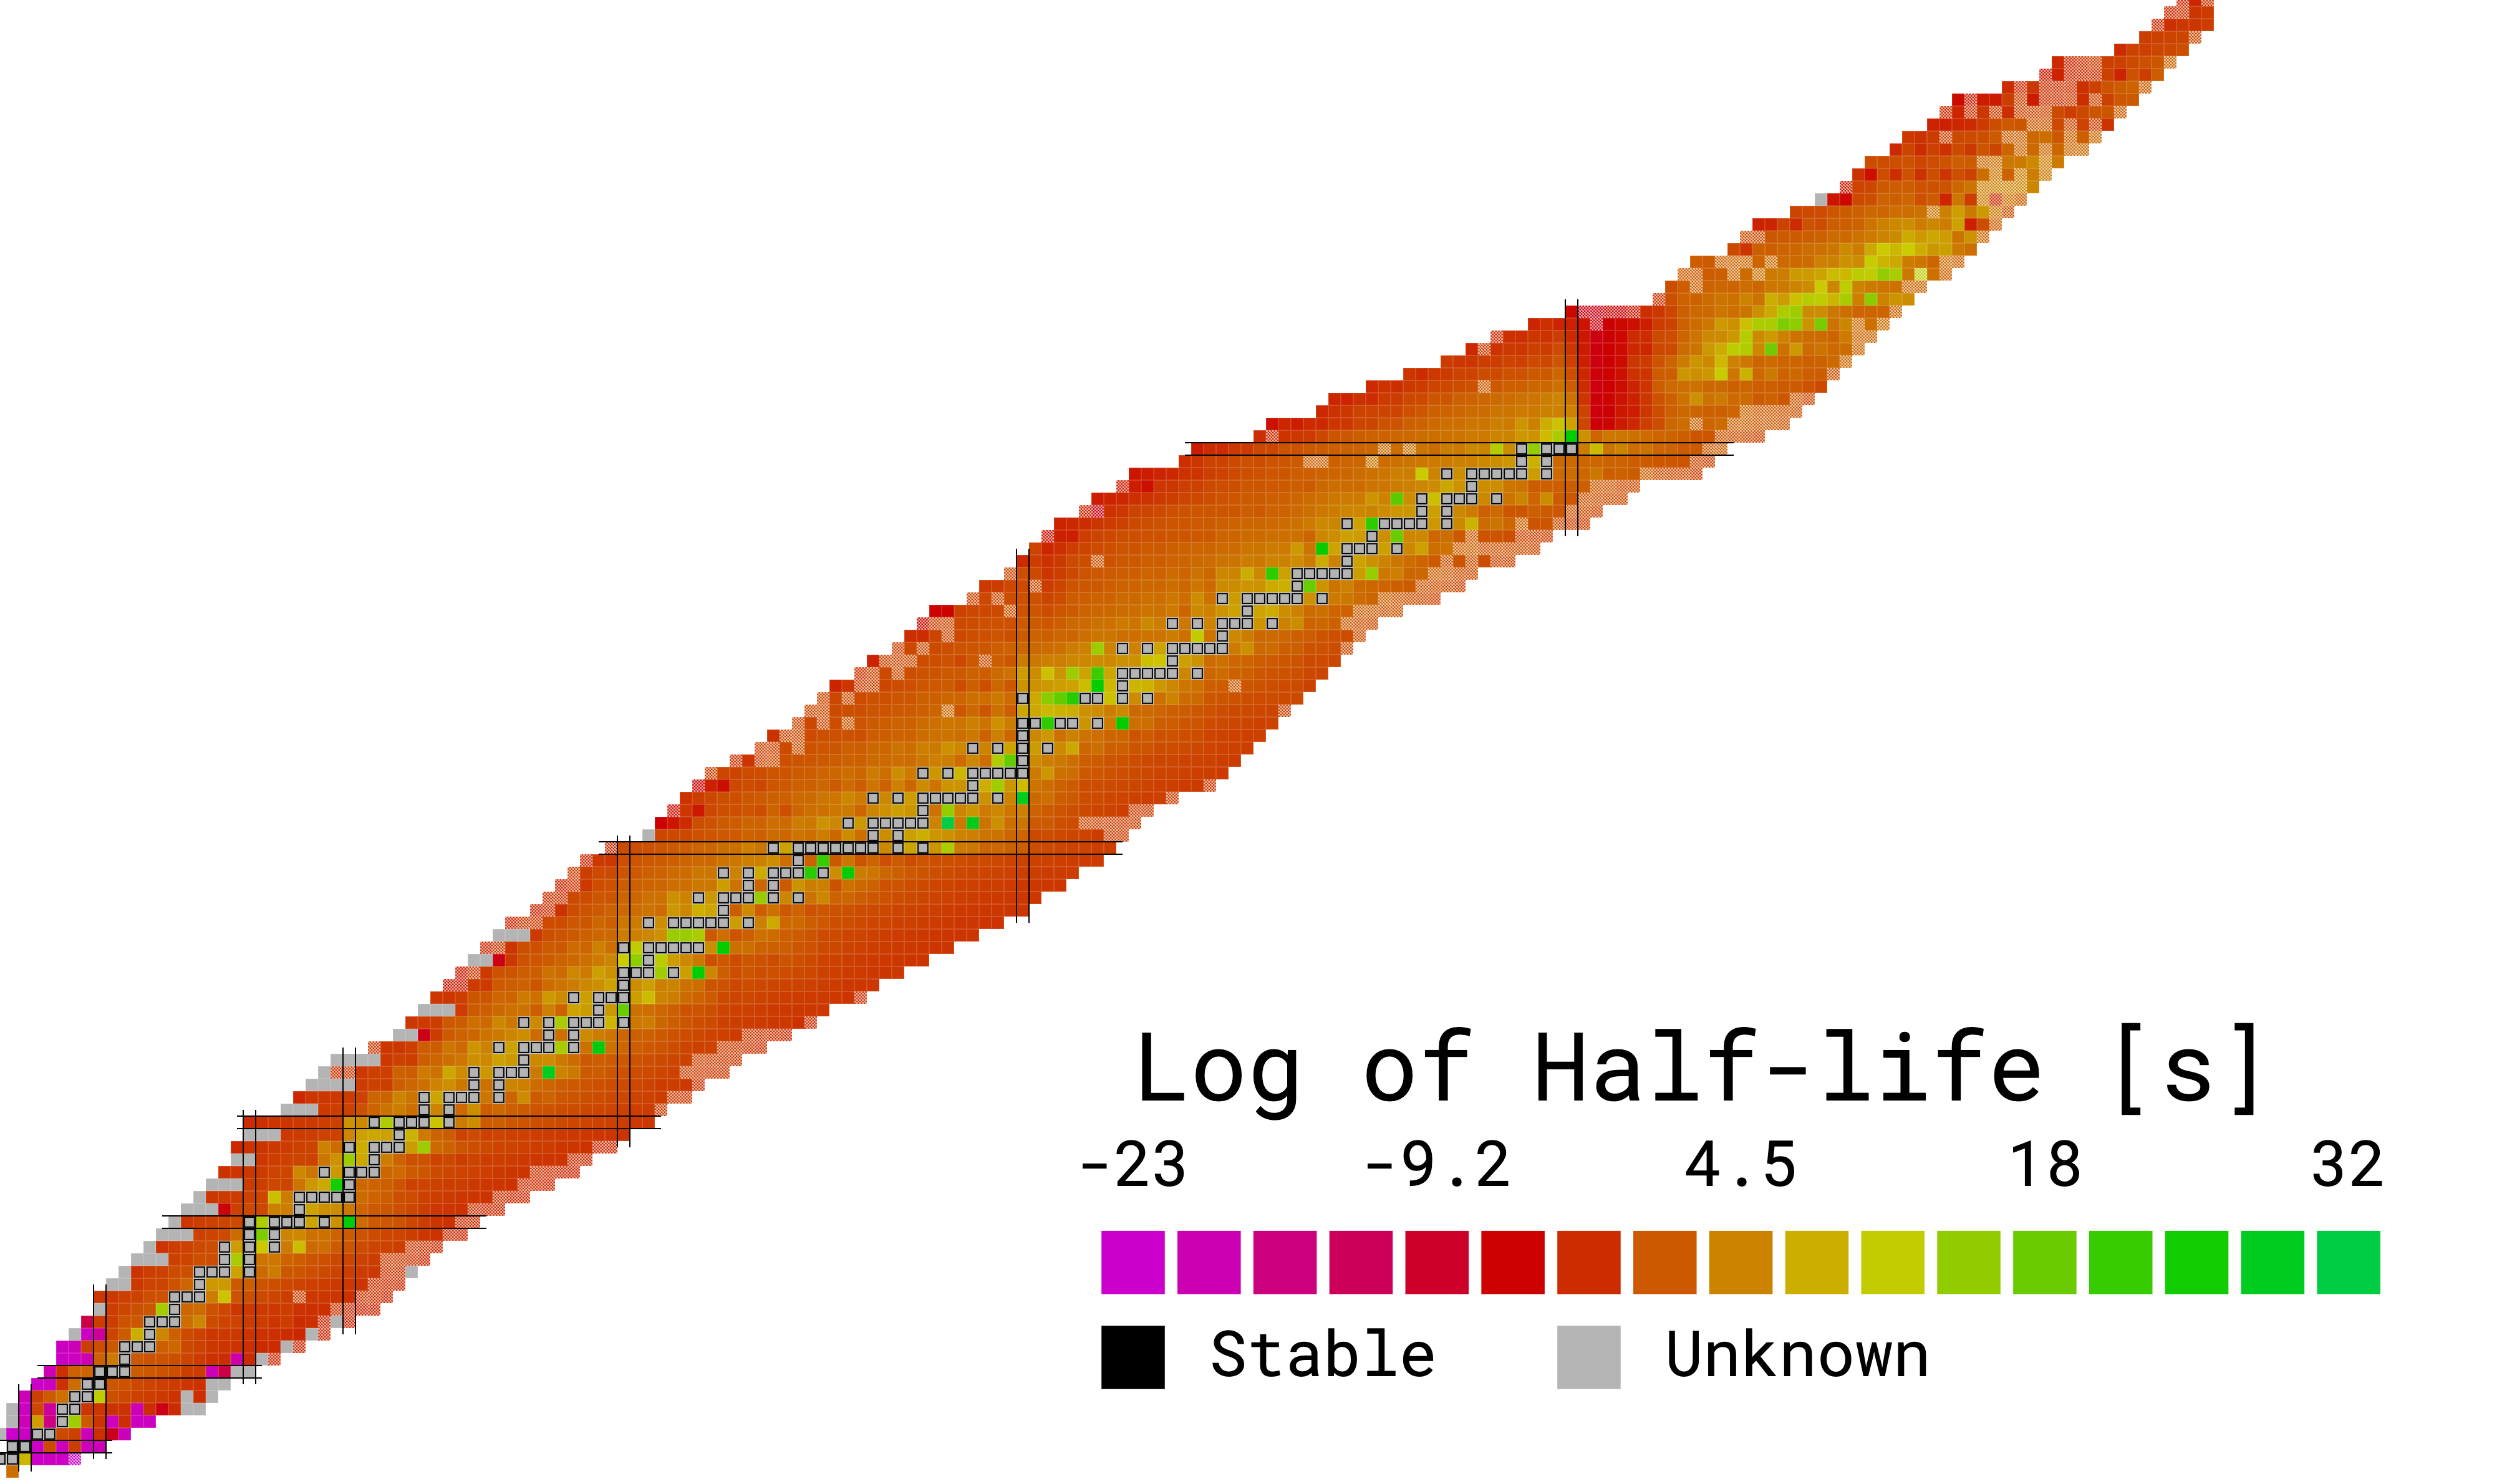
\includegraphics[width=\textwidth, height=8cm]{../plots/chart}
\caption[Chart of the nuclides]{Chart of the known nuclides. The number of protons are given along the vertical axis, and neutrons along the horizontal. The color indicates the log half-life of the nucleus. Lines of isotones and isotopes along the magic numbers are indicated by rectangles in the figure. Retrieved from Edward Simpson's \href{https://people.physics.anu.edu.au/~ecs103/chart/}{website}.}
\end{figure}

\section{Active Target Time Projection Chambers}\label{sec:attpc}

The active target time-projection chamber (AT-TPC) is a detector constructed for detection of low energy beams with a very high efficiency. It was constructed at the national superconducting cyclotron laboratory (NSCL) facility on the Michigan state university (MSU) campus. The detector is attached to the ReA3 linear accelerator which provides high quality rare isotope beams. The low-intensity of these beams necessitates a detector with high efficiency, while the low energies in the interval of $\SI[per-mode=symbol]{0.3}{\MeV \per \atomicmassunit}$ to $\SI[per-mode=symbol]{6}{\MeV \per \atomicmassunit}$ means that solid or liquid targets are not feasible (\cite{Bradt2017a})

 With the ability to provide high quality beams of rare isotopes the ReA3 re-accelerated beam facility  provides important research opportunities in nuclear physics (\cite{Kester2010}). 

 The detector consists of a cylindrical volume inserted into a solenoid magnet. The magnet, which was designed for medical imaging, applies a $\SI{2}{\tesla}$ magnetic field which is fairly uniform inside the volume (\cite{Bradt2017a}). Inside the detector the beam enters into a gas-filled volume, where the gas is specified to contain the target nucleus of interest. To record the reactions that occur in the detector a sensor plane is placed at the end of the detector, opposite the beam entrance. The sensor plane is a micromegas device consisting of an electron multiplying mesh and a plane of triangular sensors that record the impacts of impinging electrons, as described by \citet{Giomataris1996}. The pad-plane is shown in figure \ref{fig:attpc_padplane}

 \begin{figure}
\centering
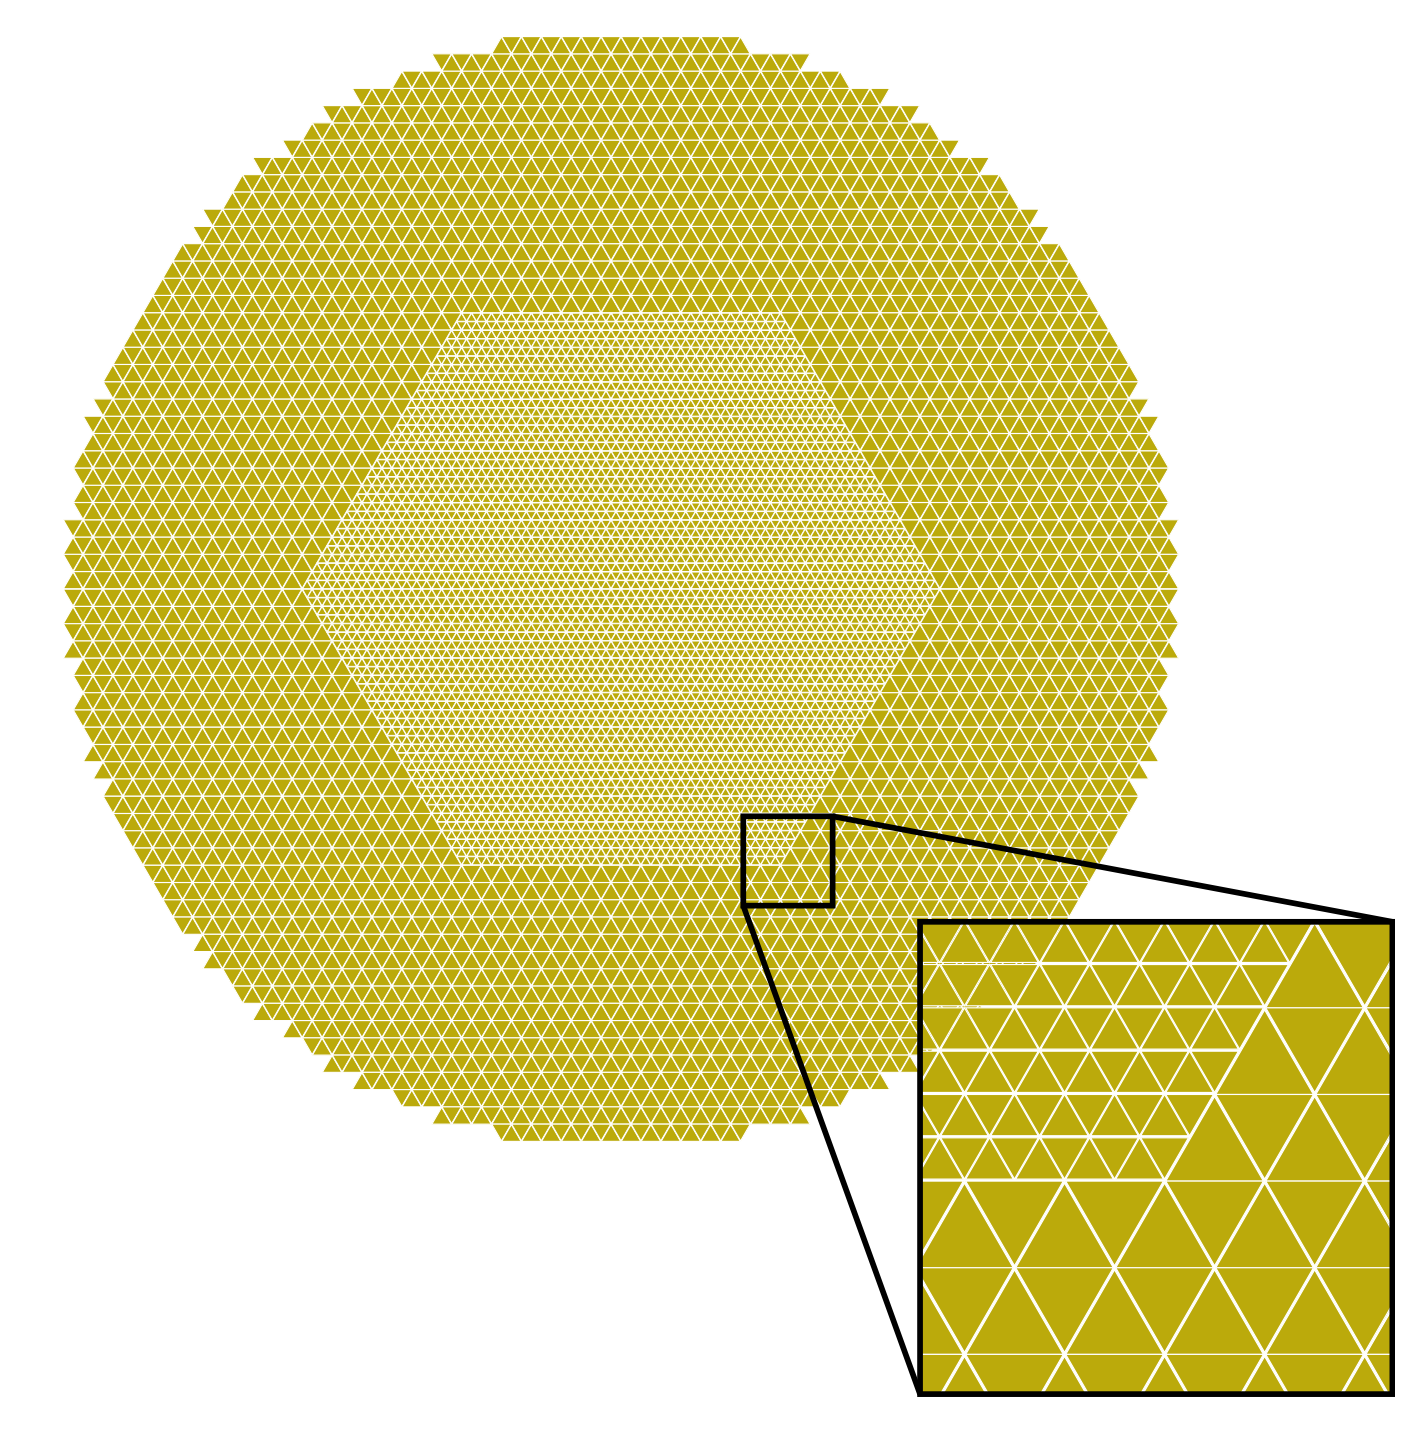
\includegraphics[width=0.5\textwidth]{../plots/at_tpc_padplane}
\caption{Figure showing the pad-plane in the AT-TPC. There are two regions of sensor-pad densities to keep the number of pads reasonable, while ensuring a high resolution in the region with high expected activity. Figure produced with the \lstinline{pytpc} package.}\label{fig:attpc_padplane}
 \end{figure}

 To get the ionization electrons from reactions in the detector to the sensor a $\SI{1e4}{\volt}$ electrical potential difference is applied between the sensor plane and the beam entrance. Furthermore, the field is kept uniform by a field cage surrounding the volume which gradually steps down the voltage (\cite{Bradt2017a}). A schematic of the AT-TPC is included in figure \ref{fig:attpc_schematic}

 \begin{figure}
 \centering
 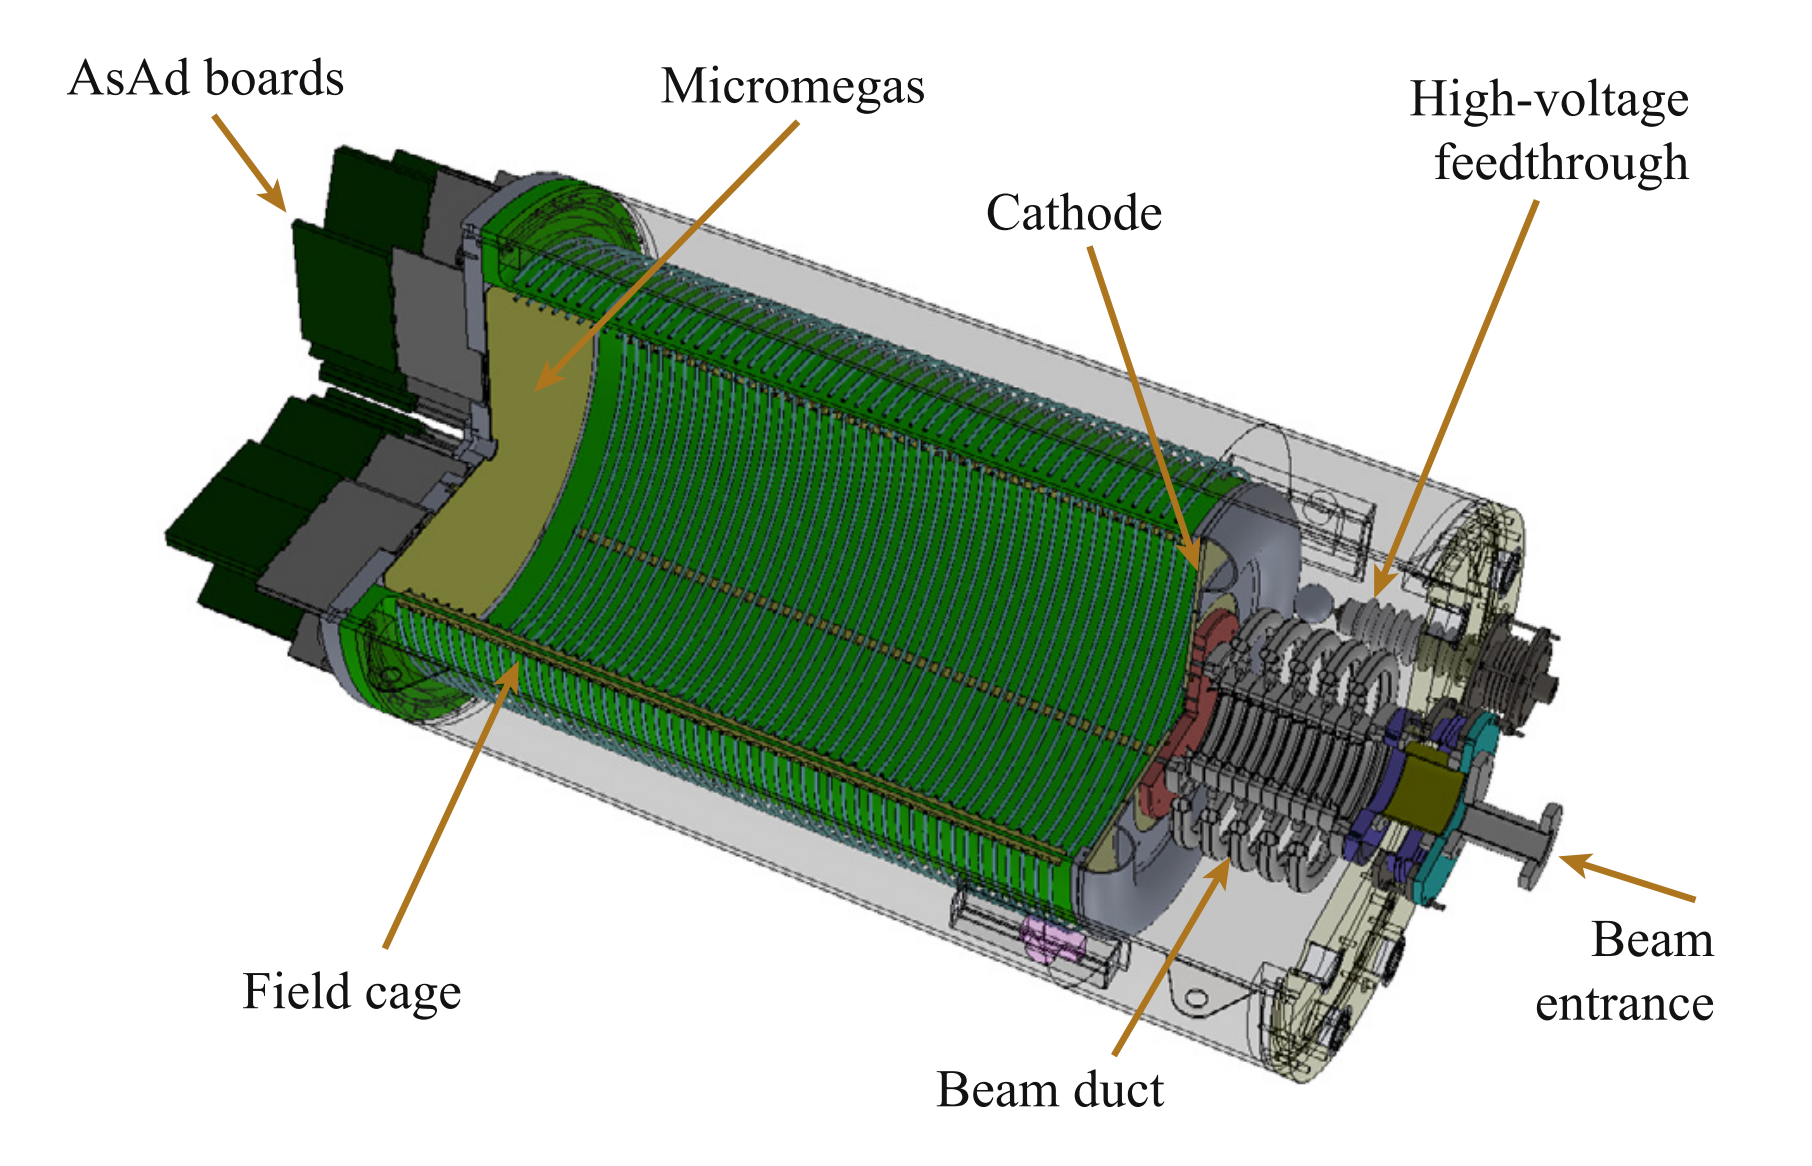
\includegraphics[width=\textwidth]{../plots/at_tpc_schematic}
 \caption[AT-TPC cross-section]{Cross section of the AT-TPC detector volume, with the outer shielding made transparent. On the right hand side the beam enters the chamber and some of the signal processing and recording equipment is shown downstream in the figure. Figure copied from \cite{Bradt2017a}}\label{fig:attpc_schematic}
 \end{figure}

The recorded signal for an event is then a collection of charge measurements from the individual sensor pads of the micromegas. In the experiment it is assumed that each pad will fire a maximum of one time per event, and as such track reconstruction begins with converting the signal from time buckets to a z coordinate. However, in this thesis we are only concerned with the x-y projection of the events. 
